\subsection{OAuth}

Az egyes API funkciók eléréséhez feltétlenül szükséges, hogy az API kliens
egy valódi felhasználót legyen képes megszemélyesíteni, erre szolgál az
OAuth protokoll, ami biztonságos autentikációt kínál \emph{3rd party}
alkalmazásoknak anélkül, hogy a felhasználónak érzékeny adatokat (jelszó, stb)
kellene az alkalmazás felé megadni.

A Twitter a protokoll 1.0a (3-legged)\cite{OAuth} verzóját használja,
ez a 2.0-ás verziónál kicsit összetettebb, azonban az \verb=oauth= node modul
teljesen elrejti a működést.

A protokoll működése az ábrán láthtó.
Az első lépés egy ún. \emph{request token} megszerzése, az alkalmazás
elküldi a saját \verb=consumer_key=-jét (és aláírja a kérést a saját
\verb=consumer_secret=-jével), amire a szerver egy \verb=request_token=-nel
válaszol. A megszerzett tokennel az alkalmazás átirányítja a felhasználót
a Twitterre, ahol engedélyeznie kell a hozzáférést (vagy belépnie a Twitterr,
ha épp ki van jelentkezve). Ha ezt megtette, visszakerül az alkalmazásba,
ami paraméterként egy újabb tokent kap (\verb=oauth_verifier=), amit
egy újabb (aláírt) kéréssel a Twitter felé kicserél egy \verb=access_token=-re
(és \verb=access_token_secret=-re).
Ezek a tokenek már elegndőek autentikált kérések indításához.

\begin{figure}[h!]
  \centering
  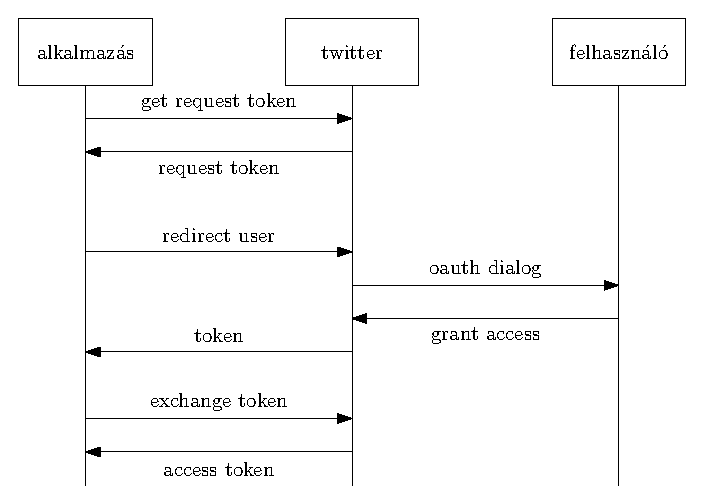
\includegraphics[width=0.95\textwidth]{figures/oauth}
  \caption{A 3-legged OAuth 1.0a autentikációs protokoll}
\end{figure}

Az azonosítás használatához regisztrálni kell a Twitter megfelelő felületén
egy új alkalmazást, majd az ott megkapott adatokkal (tokenekkel)
az autentikáció azonnal használatba vehető.

Az \verb=oauth= modul alternatívája a \verb=passport= modul, ami egy sokkal
általánosabb módszert biztosít felhasználók azonosítására (elérhető teljesen
felkonfigurált Twitter azonosítás is), azonban a \verb=koa= támogatás még
messze nem hibátlan, ezért ennek a használatát végül elvetettem.
